\documentclass{standalone}
\usepackage{tikz}




\begin{document}
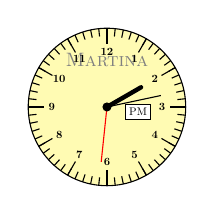
\begin{tikzpicture}
    
    \draw[fill = yellow! 30] (0,0) circle (1);
    \node[gray, scale=0.7] at (90:0.6) 
    {\textsc{Martina}} ;

    \node[fill=white, draw=black, scale=0.4] at (-9:0.4) {PM};


    \draw (0,0) -- (12:0.7); %minutero
    \draw[red] (0,0) -- (-96:0.7); %secundero
    \draw[ultra thick, line cap=round] (0,0) -- (30:0.5); %hora
    \draw[fill = black] (0,0) circle (0.05);



    %lineas de cada hora
    \foreach \ang [count=\h] in {60,30,...,-270}{

    \draw (\ang:1) -- (\ang:0.8) node[scale=0.4, pos=1.5] {\textbf{\h}};}


    %lineas de cada segundo/minuto

    \foreach \ang in {0,6,...,360}{

    \draw (\ang:1) -- (\ang:0.9);
    }    







\end{tikzpicture}   















\end{document}